

\section{Ejemplos}
    \subsection{Expresiones válidas del lenguaje}
        \begin{enumerate}
            \item \textbf{\texttt{2+(\{\{(\{C/B\})\}/C\})}}

            \underline{Output}:
            \begin{center}                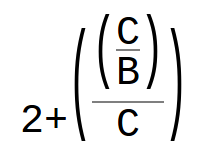
\includegraphics[width=3cm,keepaspectratio]{Ej1}
            \end{center}

            \underline{AST generado: } \\
            \texttt{\seqsplit{Concat(Concat(Chr(2),Chr(+)),GroupedPar(DivExpr(GroupedPar(DivExpr(Chr(C),Chr(B))),Chr(C))))}}

            \item
            \textbf{\texttt{(\{(A/B)(A/B)\}\^{}\{((A/B)(A/B)\_{}\{(A\_{}B)\})\})(A\_{}\{B\^{}\{B\^{}\{B\}\}\})}}

            \underline{Output}:
            \begin{center}                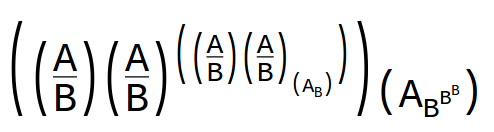
\includegraphics[width=8.5cm,keepaspectratio]{Ej2}
            \end{center}

            \underline{AST generado: } \\
            \texttt{\seqsplit{Concat(GroupedPar(SuperSub(Concat(GroupedPar(DivExpr(Chr(A),Chr(B))),GroupedPar(DivExpr(Chr(A),Chr(B)))), GroupedPar(Concat(GroupedPar(DivExpr(Chr(A),Chr(B))),SubSuper(GroupedPar(DivExpr(Chr(A),Chr(B))), LambdaExpr, GroupedPar(SubSuper(Chr(A), LambdaExpr, Chr(B)))))), LambdaExpr)),GroupedPar(SubSuper(Chr(A), LambdaExpr, SuperSub(Chr(B), SuperSub(Chr(B), Chr(B), LambdaExpr), LambdaExpr))))}}

            \item
            \textbf{(Ax+B)\super \{A\_{}B\}(A)\sub \{A\super A\}}

            \underline{Output}:
            \begin{center}                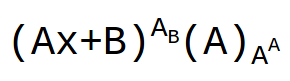
\includegraphics[width=5cm,keepaspectratio]{Ej3}
            \end{center}

            \underline{AST generado: } \\
            \texttt{\seqsplit{Concat(SuperSub(GroupedPar(Concat(Concat(Concat(Chr(A),Chr(x)),Chr(+)),Chr(B))), SubSuper(Chr(A), LambdaExpr, Chr(B)), LambdaExpr),SubSuper(GroupedPar(Chr(A)), LambdaExpr, SuperSub(Chr(A), Chr(A), LambdaExpr)))}}

            \item
            \textbf{\texttt{\{a\^{}2\_{}1+a\^{}2\_{}2+...+a\^{}2\_{}n\}/\{||(a\_{}1,...,a\_{}n)||\}}}

            \underline{Output}:
            \begin{center}                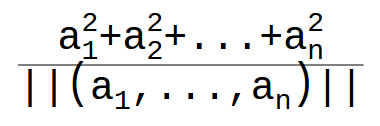
\includegraphics[width=6cm,keepaspectratio]{imagenes/Ej4.png}
            \end{center}

            \underline{AST generado: } \\
            \texttt{\seqsplit{DivExpr(Concat(Concat(Concat(Concat(Concat(Concat(Concat(Concat(SuperSub(Chr(a), Chr(2), SubSuffix(Chr(1))),Chr(+)),SuperSub(Chr(a), Chr(2), SubSuffix(Chr(2)))),Chr(+)),Chr(.)),Chr(.)),Chr(.)),Chr(+)),SuperSub(Chr(a), Chr(2), SubSuffix(Chr(n)))),Concat(Concat(Concat(Concat(Chr(|),Chr(|)),GroupedPar(Concat(Concat(Concat(Concat(Concat(Concat(SubSuper(Chr(a), LambdaExpr, Chr(1)),Chr(,)),Chr(.)),Chr(.)),Chr(.)),Chr(,)),SubSuper(Chr(a), LambdaExpr, Chr(n))))),Chr(|)),Chr(|)))}}

            \item
            \textbf{\texttt{\{\{A\^{}\{A\^{}\{A\^{}\{A\}\}\}\_{}n\}/\{B\^{}\{B\^{}\{B\}\}\_{}m\}\}+A+B}}

            \underline{Output}:
            \begin{center}                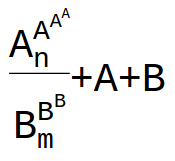
\includegraphics[width=3cm,keepaspectratio]{imagenes/Ej5.png}
            \end{center}

            \underline{AST generado: } \\ \texttt{\seqsplit{Concat(Concat(Concat(Concat(DivExpr(SuperSub(Chr(A), SuperSub(Chr(A), SuperSub(Chr(A), Chr(A), LambdaExpr), LambdaExpr), SubSuffix(Chr(n))),SuperSub(Chr(B), SuperSub(Chr(B), Chr(B), LambdaExpr), SubSuffix(Chr(m)))),Chr(+)),Chr(A)),Chr(+)),Chr(B))}}
        \end{enumerate}
    \subsection{Expresiones inválidas del lenguaje}
        \begin{enumerate}
            \item
            \textbf{\texttt{2+(\{\}}} (se abre un paréntesis que nunca se cierra).

            \item
            \textbf{\texttt{(A/B\})}} (se cierra una llave que nunca se abre).

            \item
            \textbf{\texttt{A\^{}\{b+1\}\_{}}}  (subíndice vacío)

            \item
            \textbf{\texttt{A4\{\}\^{}}} (superíndice vacío)

            \item (cadena vacía)

            \item
            \textbf{\texttt{A\^{}A\^{}A}} (asociatividad de superíndices)

            \item
            \textbf{\texttt{A\^{}B\_{}C\^{}D}} ($>1$ superíndices en el mismo \quotes{scope} de paréntesis/llaves $\Rightarrow$ asociatividad implícita de superíndices)
        \end{enumerate}
